\documentclass[11pt]{article}

\def\mainroot{ell_1}

\usepackage[top=1in, bottom=1in, left=1in, right=1in]{geometry}

\usepackage[compact]{titlesec}

\usepackage{xcolor}
\definecolor{pykeyword}{HTML}{000088}
\definecolor{pyidentifier}{HTML}{000000}
\definecolor{pystring}{HTML}{008800}
\definecolor{pynumber}{HTML}{FF4000}
\definecolor{pycomment}{HTML}{880000}

\usepackage{listings}
\lstset{language=Python,
	basicstyle=\ttfamily\small,
	tabsize=4,
	showstringspaces=false,
	keywordstyle=\color{pykeyword},
	identifierstyle=\color{pyidentifier},
	stringstyle=\color{pystring},
	numberstyle=\color{pynumber},
	commentstyle=\color{pycomment}
}

\usepackage{algorithm}
\usepackage{algpseudocode}

\usepackage{graphicx}

\title{CSE 537 Assignment 1 Report: Peg Solitaire}

\author{
Remy Oukaour \\
	{\small SBU ID: 107122849}\\
	{\small \texttt{remy.oukaour@gmail.com}}
\and
Jian Yang \\
	{\small SBU ID: 110168771}\\
	{\small \texttt{jian.yang.1@stonybrook.edu}}
}

\date{Thursday, September 24, 2015}

\raggedbottom

\begin{document}

\maketitle

\section{Introduction}

This report describes our submission for assignment 1 in the CSE 537 course on
artificial intelligence. Assignment 1 requires us to implement three algorithms
for solving a game of Peg Solitaire: iterative-deepening depth-first search
(ID-DFS), and A* search with two different heuristics. In this report, we
discuss the implementation details and compare the performance of six solutions
(ID-DFS and five A* heuritsics, of which we settled on two).

\section{Implementation}

We were given four Python code files implementing the assignment framework:
\(readGame.py\), \(pegSolitaireUtils.py\), \(search.py\), and \(pegSolitaire.py\).
We did not need to edit \(readGame.py\) or \(pegSolitaire.py\), but only had to
implement utility classes and methods in \(pegSolitaireUtils.py\) and the search
algorithms in \(search.py\).

\subsection{Data structures}

The original data structure given in \(pegSolitaireUtils.py\) was a single
class \(game\) containing the game state as a 2-dimensional 7 $\times$ 7 array of
integers, a trace of the moves taken to reach that state, and an overall count
of the nodes expanded by the search algorithm. To make the implementation more
clear, we split this into two classes: \(game\), a singleton class storing
overall state for a search (the original game state, final move trace, and
expanded node count), and \(gameNode\), a class which a search algorithm can
repeatedly create as it explores the game tree.

The \(gameNode\) class contains some optimizations. We flattened the game state
into a 1-dimensional array of 49 integers to speed up indexing and simplify
copying. Thus, an index \(gameState[i][j]\) would become \(gameState[i*7+j]\).
(We did not change the state representation of \(game\), only of \(gameNode\).)
We also cache two pieces of data when a \(gameNode\) is created: a count of
pegs remaining on the board, and a \(key\) state chosen from the eight symmetric
states under rotation and reflection. This data is used by our search algorithms
to prune search trees.

\subsection{Utility methods}

We were required to implement four utility methods in \(pegSolitaireUtils.py\):

\begin{enumerate}

\item \(is\_corner(self, pos)\):

\lstset{language=Python}
\begin{lstlisting}[frame=single]
def is_corner(self, pos):
	"""
	Return whether a position is a corner/wall,
	i.e. not a hole or peg.
	"""
	return 0 <= pos < 49 and self.state[pos] != -1
\end{lstlisting}

In implementation, we actually used another function
\(\_\_getitem\_\_(self, pos)\) instead:

\lstset{language=Python}
\begin{lstlisting}[frame=single]
def __getitem__(self, pos):
	"""
	node[pos] is bounds-checked shorthand for node.state[pos].
	"""
	return self.state[pos] if 0 <= pos < 49 else -1
\end{lstlisting}

\item \(is\_validMove(self, oldPos, direction)\):

\lstset{language=Python}
\begin{lstlisting}[frame=single]
def is_validMove(self, oldPos, direction):
	"""
	Return whether it is valid to move a peg from a given
	position in a given direction. The position must have a
	peg, the destination must be empty, and the intermediate
	position must have another peg.
	"""
	midPos = self.getNextPosition(oldPos, direction)
	newPos = self.getNextPosition(midPos, direction)
	# 1 is a peg, and 0 is a hole
	# Since oldPos is valid, don't use bounds-checked
	# indexing for it
	return (self.state[oldPos] == self[midPos] == 1
		and self[newPos] == 0)
\end{lstlisting}

\item \(getNextPosition(self, oldPos, direction)\):

\lstset{language=Python}
\begin{lstlisting}[frame=single]
@staticmethod
def getNextPosition(oldPos, direction):
	"""
	Return the new position after moving in the given
	direction (-7 is north/up, 1 is east/right, 7 is south/
	down, and -1 is west/left). Invalid movements outside
	the bounds of the board will return positions such that
	is_corner(position) returns True.
	"""
	newPos = oldPos + direction
	# If direction is 7 or -7 (changing rows),
	# newPos is already correct
	return (newPos if direction == 7 or direction == -7 or
	# If direction is 1 or -1 (changing columns),
	# the row should not change
		newPos // 7 == oldPos // 7 else -1)
\end{lstlisting}

\item \(getNextState(self, oldPos, direction)\):

\lstset{language=Python}
\begin{lstlisting}[frame=single]
def getNextState(self, oldPos, dir, pegSol):
	"""
	Return a child node of the current one, created by a
	given valid move. The given game has its count of
	expanded nodes incremented.
	"""
	pegSol.nodesExpanded += 1
	if not self.is_validMove(oldPos, direction):
		print "Error, You are not checking for valid move"
		exit(0)
	midPos = self.getNextPosition(oldPos, direction)
	newPos = self.getNextPosition(midPos, direction)
	# x[:] makes a copy of x (necessary to avoid mutating
	# self.state when updating childState)
	childState = self.state[:]
	childState[oldPos] = 0 # The peg moves from here
	childState[midPos] = 0 # The jumped-over peg is removed
	childState[newPos] = 1 # The peg moves to this hole
	# Convert positions back into pairs for printing
	childTrace = self.trace + [(oldPos // 7, oldPos \% 7),
		(newPos // 7, newPos \% 7)]
	return gameNode(childState, childTrace,
		self.pegCount - 1, self.heuristic)
\end{lstlisting}

\end{enumerate}

\subsection{Search functions}

We were required to implement our search functions and heuristics in
\(search.py\).

We implemented ID-DFS straightforwardly, based on figure 3.17 (section 3.4,
page 88) and figure 3.18 (section 3.4, page 89) in the textbook. However, we
also maintain a set of explored nodes (modulo symmetry) to avoid revisiting,
which helps prune the search tree.

We implemented A* based on figure 3.14 (section 3.4, page 84) in the textbook.
However, we take the set of \(explored\) nodes modulo symmetry to further prune
the search tree. (One game state can be solved if and only if its seven
symmetrical states can be solved, so when one has been expanded the other
seven can be pruned.)

\subsubsection{First A* heuristic}

\lstset{language=Python}
\begin{lstlisting}[frame=single]
def heuristicOne(node):
	"""
	This heuristic counts the number of "dangling" pegs (those
	without any neighbors) and adds it to twice the number of
	pegs remaining on the board.

	We penalize dangling pegs because they cannot be removed
	without first moving another peg to a neighboring hole,
	which may not be possible.
	"""
	num_dangling = 0
	for i in xrange(49):
		if node.state[i] != 1: continue
		for direction in [7, 1, -7, -1]:
			if node[i + direction] == 1:
				break
		else:
			num_dangling += 1
	return node.pegCount * 2 + num_dangling
\end{lstlisting}

\subsubsection{Second A* heuristic}

\lstset{language=Python}
\begin{lstlisting}[frame=single]
def heuristicTwo(node):
	"""
	This heuristic sums the estimated difficulty of removing
	each peg and adds it to twice the number of pegs remaining
	on the board.

	We chose the difficulty values after some trial and error.
	The outer four areas of the board are generally less
	maneuverable than the center, and further from the eventual
	goal of the very central hole. This applies especially to
	the eight outer corners, which have fewer neighbors to jump
	over. The four inner corners are only slightly easier, since
	they have more neighbors but are still not in the ideal rows
	or columns. (Note that pegs in the outer and inner corners
	can only move within those positions, never to a non-corner
	hole.) The center peg is the end goal of the game, but prior
	to that having a peg sit there is not quite useful (since if
	you are left with two pegs and one is in the center, the
	game is unsolvable).
	"""
	difficulties = [
		0, 0, 4, 1, 4, 0, 0,
		0, 0, 1, 1, 1, 0, 0,
		4, 1, 2, 0, 2, 1, 4,
		1, 1, 0, 1, 0, 1, 1,
		4, 1, 2, 0, 2, 1, 4,
		0, 0, 1, 1, 1, 0, 0,
		0, 0, 4, 1, 4, 0, 0,
	]
	return node.pegCount * 2 + sum(difficulties[k]
		for k in xrange(49) if node.state[k] == 1)
\end{lstlisting}

\subsubsection{Other A* heuristics}

We tested various other heuristics before settling on our chosen two. One of
them was a baseline heuristic that simply returned the number of remaining
pegs. The other three were all variations on \(heuristicTwo\) with a different
\(difficulties\) array.

\begin{enumerate}

\item Manhattan distance from center neighbors:

\begin{lstlisting}[frame=single]
distances = [
	5, 4, 3, 2, 3, 4, 5,
	4, 3, 2, 1, 2, 3, 4,
	3, 2, 1, 0, 1, 2, 3,
	2, 1, 0, 1, 0, 1, 2,
	3, 2, 1, 0, 1, 2, 3,
	4, 3, 2, 1, 2, 3, 4,
	5, 4, 3, 2, 3, 4, 5
]
\end{lstlisting}

\item Alternative difficulties \#1:

\lstset{language=Python}
\begin{lstlisting}[frame=single]
difficulties = [
	0, 0, 4, 0, 4, 0, 0,
	0, 0, 0, 0, 0, 0, 0,
	4, 0, 3, 0, 3, 0, 4,
	0, 0, 0, 1, 0, 0, 0,
	4, 0, 3, 0, 3, 0, 4,
	0, 0, 0, 0, 0, 0, 0,
	0, 0, 4, 0, 4, 0, 0
]
\end{lstlisting}

\item Alternative difficulties \#2:

\lstset{language=Python}
\begin{lstlisting}[frame=single]
difficulties = [
	0, 0, 1, 1, 1, 0, 0,
	0, 0, 1, 1, 1, 0, 0,
	1, 1, 0, 0, 0, 1, 1,
	1, 1, 0, 0, 0, 1, 1,
	1, 1, 0, 0, 0, 1, 1,
	0, 0, 1, 1, 1, 0, 0,
	0, 0, 1, 1, 1, 0, 0
]
\end{lstlisting}

\end{enumerate}

\section{Results}

\subsection{Test cases}

Our first test case was the given \(game.txt\), a board with 6 pegs in a
cross shape.

We wrote ten more test cases manually based on actual game boards that people
play, such as a 9-peg plus shape, a 16-peg pyramid, a 24-peg diamond, or the
32-peg ``central game'' with only one hole in the center.

We also created 100 random test cases with between 2 and 21 pegs, by
implementing a generator for random valid test cases. It works by starting
with the goal state (only one peg in the center) and randomly picking valid
backward moves that could have reached that state. In pseudocode:

\begin{algorithm}
\caption{Random test case generator}
\label{random_alg}
\begin{algorithmic}[1]
	\State{$numSteps \gets$ pick a random number between 1 and 33 }
	\State{$boardState \gets$ goal board state, with only one peg in the center }
	\For{$j \gets 1$ to $numSteps$}
		\State{$validStartPos, validDirection \gets$ pick a random valid move}
		\State{$boardState[validStartPos] \gets$ 0}
		\State{$boardState[validStartPos + validDirection] \gets$ 1}
		\State{$boardState[validStartPos + validDirection + validDirection] \gets$ 1}
	\EndFor
	\State \Return{$board\_state$}
\end{algorithmic}
\end{algorithm}

\subsection{Benchmarks}

We compared the performance of our different search algorithms on a few test cases:

\begin{enumerate}
\item The given 6-peg \(game.txt\)
\item The 32-peg central game
\item The mean expanded node count of all 110 test boards
\item The median count of all 110 test boards
\end{enumerate}

The performance results for our different search algorithms are shown in table \ref{tab_perf}:

\begin{table}[h!]
\centering
\begin{tabular}{| l | r | r | r | r | r | r | r | r |}
\hline
\textbf{Test case} & \textbf{ID-DFS} & \textbf{A*1} & \textbf{A*2} & \textbf{A*Base} &
	\textbf{A*Manhattan} & \textbf{A*Diff1} & \textbf{A*Diff2} \\
\hline
game.txt & 50 & 16 & 13 & 13 & 19 & 13 & 19 \\
\hline
Central game & MemoryError & 4,713,300 & 103,402 & 26,807 & 1,801,655 & 170 & 530,402 \\
\hline
Mean & 1,979,736 & 47,084 & 3,388 & 5,146 & 19,201 & 4,394 & 8,917 \\
\hline
Median & 6,417 & 74 & 98 & 92 & 95 & 128 & 114 \\
\hline
\end{tabular}
\caption{Expanded node counts for all algorithms in different test cases}
\label{tab_perf}
\end{table}

We also tested each algorithm on a board with no solution (two noncontiguous pegs).
They all succeeded in printing ``Impossible to solve'' instead of a solution move
trace, without crashing or infinitely looping.

The heuristics A*2, A*Manhattan, A*Diff1, and A*Diff2 were conceptually very
similar, so we only wanted to submit one of them. Our tests found that A*2 was
the most efficient: it had the lowest mean count (of all the algorithms), and
while A*Manhattan had a slightly lower median count, it could not solve the
central game quickly enough.

We never intended to submit A*Base as a heuristic, since it was so simple, so we
were surprised to see it perform as well as it did. It had a competitive mean
expanded node count and the lowest median count. We hypothesize that our more
complicated heuristics are better for particular game boards, but not for every
possible random board that we were trying.

\subsection{Performance notes}

In our testing, we found an interesting phenomenon. When enumerating valid moves
from a particular position in a particular game state, there can be at most four
moves (north, south, east, and west). For several large test cases, if we test
those four directions in a different order, performance can significantly vary.
There are $4!$, or 24 possible orders, so we tested all 24 of them against all
six search algorithms. The 24 possibilities break down into two categories:
``opposite-order first'' (such as ``north, south, east, west'') and ``orthogonal-
order first'' (such as ``north, east, south, west''). By plotting the results in
figure \ref{fig_boxplot}, it is clear that the ``orthogonal-order first'' category
had slightly better performance.

\begin{figure}[h!]
\centering
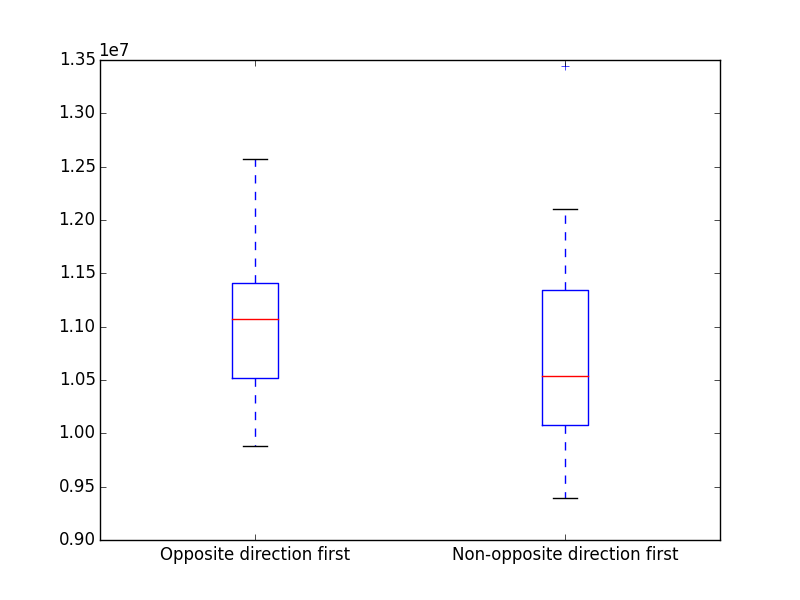
\includegraphics[height=3.5in, width=4.5in]{figs/boxplot.png}
\caption{Box plot for two sets of summations}
\label{fig_boxplot}
\end{figure}

\section{Conclusion}

TODO: conclusion

\end{document}
